%----------------------------------------------------------------------------------------
%	PART
%----------------------------------------------------------------------------------------

\part{Preliminaries}

%----------------------------------------------------------------------------------------
%	CHAPTER 1
%----------------------------------------------------------------------------------------

\chapterimage{chapter_head_2} % Chapter heading image

\chapter{Processors}

\section{Introduction}\index{Introduction}

Whenever we are playing any game like \textit{Crysis 3}, and the frame rate stutters, we exclaim, "\textit{This computer is so slow!}", without normally realizing the implications of what we say. What does it mean when we say a computing device is slow or fast ? How does a computing device actually perform computational tasks and instructions ?

Some of us may be aware that these computational tasks are performed by what is known as a Central Processing Unit or as are more commonly called, a Processor. 

\textbf{A processor carries out the instructions of a computer program by performing the basic arithmetic, logical, control and input/output (I/O) operations specified by the instructions.}

\begin{remark}
We would like to mention that not all computational tasks are performed by Processors, some tasks are delegated to other modules like Graphical Processing Units (GPU's), but we'll keep that out of scope of our discussion.
\end{remark}

The major aim of this book would be to understand how processors work and also learn the basic design principles that govern the design of a processor. 

We will be looking at processor design through a simple design and would study about various building blocks concerning that design. We would also learn some basic instructions that are a part of the processor design and also learn how these instructions are implemented and run in the processor.

For a hands on experience, we will also be writing some instructional level (called assembly) code for the processor design (on a simulator) and understanding how processors work at a very low level. As an aside, we'll also learn how our assembly code is translated to processor readable code and review different ways this is assembly is performed.

\newpage

%------------------------------------------------

\section{Brief History}\index{Brief History}

\begin{wrapfigure}{r}{0.4\textwidth}
\caption{EDVAC at Ballistics Research Lab}
\label{fig:edvac}
\centering
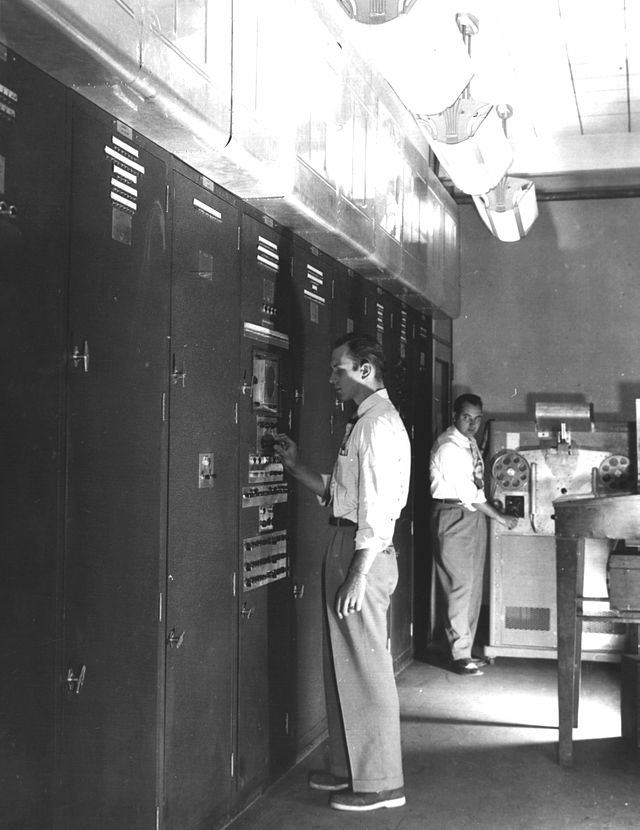
\includegraphics[width=0.4\textwidth]{EDVAC}
\end{wrapfigure}

Early computers like ENIAC were not programmable in nature in the sense of the word as we know it. To "program" these computers, one had to physically rewire them, which obviously was a very cumbersome process. Around the same time, the concept of "stored program" was floated around by John von Neumann through a report on EDVAC. 

EDVAC was designed to perform a certain basic instructions and programs written for EDVAC were to be stored in high-speed computer memory rather than specified by the physical wiring, which made writing programs and performing computational tasks much less cumbersome. These developments motivated the development of modern processors. 

Another architecture was popular in those times, known as the Harvard architecture. The key difference between the von Neumann and Harvard architectures is that the latter separates the storage and treatment of CPU instructions and data, while the former uses the same memory space for both. 

\begin{remark}
Most modern CPUs are primarily von Neumann in design, but CPUs with the Harvard architecture are seen mostly in embedded applications.
\end{remark}

With the advent of transistors, processor design grew increasingly more complex. Transistor-based computers had several distinct advantages over their predecessors. With increased reliability and lower power consumption, the CPUs operated at much higher speeds because of the short switching time of a transistor (from high to low and vice versa). 

\begin{wrapfigure}{l}{0.4\textwidth}
\caption{AL1, one of the first microprocessors}
\label{fig:edvac}
\centering
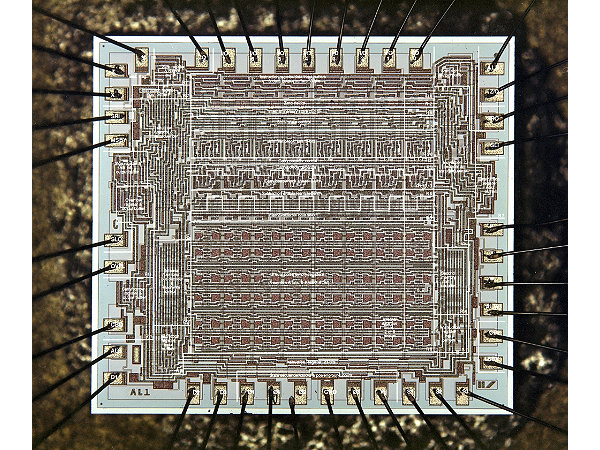
\includegraphics[width=0.4\textwidth]{al1}
\end{wrapfigure}

Transition was made from combining different components to building a System-on-Chip (SoC).  The integrated circuit (IC) allowed a large number of transistors to be manufactured on a "chip". Initially only basic circuits like NOR gates were miniaturized into ICs. CPUs based upon these IC's (building blocks) are generally referred to as small-scale integration (SSI) devices.

Further developments led to invention of techniques like Large Scale Integration, Very Large Scale Integration and finally, the Microprocessor. Previous generations of CPUs were implemented as discrete components and numerous small IC's on one or more circuit boards. Microprocessors, on the other hand, are CPUs manufactured on a very small number of IC's; usually just one.

\begin{remark}
Gordon E. Moore, the co-founder of Intel observed that the number of transistors in a dense integrated circuit doubles approximately every two years.
\end{remark}

While the complexity, size, construction, and general form of CPUs have changed enormously, the basic design and function hasn't changed much. Nearly all CPUs are von Neumann stored program machines.

%------------------------------------------------

\section{Basic Structure and Operation}\index{Basic Structure and Operation}

